\documentclass{beeper}

\usepackage{fontawesome}
\usepackage{etoolbox}
\usepackage{textcomp}
\usepackage[nodisplayskipstretch]{setspace}
\usepackage{xspace}
\usepackage{verbatim}
\usepackage{multicol}
\usepackage{soul}
\usepackage{attrib}

\usepackage{amsmath,amssymb,amsthm}

\usepackage[linesnumbered,commentsnumbered,ruled,vlined]{algorithm2e}
\newcommand\mycommfont[1]{\footnotesize\ttfamily\textcolor{blue}{#1}}
\SetCommentSty{mycommfont}
\SetKwComment{tcc}{ \# }{}
\SetKwComment{tcp}{ \# }{}

\usepackage{siunitx}

\usepackage{tikz}
\usepackage{pgfplots}
\usetikzlibrary{decorations.pathreplacing,calc,arrows.meta,shapes,graphs}

\setmainfont{Open Sans Light}
\usefonttheme{serif}

\makeatletter
\patchcmd{\beamer@sectionintoc}{\vskip1.5em}{\vskip0.5em}{}{}
\makeatother

% Math stuffs
\newcommand{\Z}{\mathbb{Z}}
\newcommand{\R}{\mathbb{R}}
\newcommand{\N}{\mathbb{N}}
\newcommand{\lcm}{\text{lcm}}
\newcommand{\Inn}{\text{Inn}}
\newcommand{\Aut}{\text{Aut}}
\newcommand{\Ker}{\text{Ker}\ }
\newcommand{\la}{\langle}
\newcommand{\ra}{\rangle}

\newcommand{\yournewcommand}[2]{Something #1, and #2}

\newenvironment{question}[1]{\par\textbf{Question #1.}\par}{}

\newcommand{\pmidg}[1]{\parbox{\widthof{#1}}{#1}}
\newcommand{\splitslide}[4]{
    \noindent
    \begin{minipage}{#1 \textwidth - #2 }
        #3
    \end{minipage}%
    \hspace{ \dimexpr #2 * 2 \relax }%
    \begin{minipage}{\textwidth - #1 \textwidth - #2 }
        #4
    \end{minipage}
}

\newcommand{\frameoutput}[1]{\frame{\colorbox{white}{#1}}}

\newcommand{\tikzmark}[1]{%
\tikz[baseline=-0.55ex,overlay,remember picture] \node[inner sep=0pt,] (#1)
{\vphantom{T}};
}

\newcommand{\braced}[3]{%
    \begin{tikzpicture}[overlay,remember picture]
        \draw [thick,decorate,decoration={brace,raise=1ex,amplitude=4pt},blue] (#2.south west-|T1.south west) -- node[anchor=west,left,xshift=-1.8ex,text=olive]{#3} (#1.north west-|T1.south west);
    \end{tikzpicture}
}

\title{Matrix Cryptographic Key Infrastructure}
\author{Sumner Evans}
\institute{Beeper (Automattic)}
\date{21 September 2024}

\begin{document}

\begingroup
\def\insertframenumber{\relax}
\begin{frame}
    \titlepage

    \note[item]{
        Hello, my name is Sumner, I'm a software engineer at Automattic working
        on Beeper and today I'm going to be talking about cryptographic key
        infrastructure in Matrix.
    }
    \note[item]{
        End-to-end encryption is one of the things which brought me to Matrix,
        and I'm sure that it's one of the factors that brought many of you to
        Matrix as well.
    }
    \note[item]{
        However, Matrix's user experience with cryptography is often confusing.
        I mainly blame the other chat networks for their incompetence. Most
        other chat networks don't even provide any cryptographically-guaranteed
        security and privacy. Some networks provide encryption in a way that
        does not truly leave the user in control of their keys. Only a few
        networks (Signal) truly leave the user in control, and their UX is
        arguably worse than Matrix.
    }
    \note[item]{
        In this talk, my goal is to discuss the cryptographic key
        \textit{infrastructure} in Matrix. What do I mean by ``infrastructure''?
        I mean all of the features which support key sharing and identity
        verification, but don't actually themselves provide security. You can
        think of this talk as discussing the ``UX layer of cryptography in
        Matrix''. None of the things that I'm going to discuss are strictly
        necessary for ensuring secure E2EE communication, but without them,
        Matrix' UX would be horrible.
    }
\end{frame}
\endgroup

\begin{frame}{Why Cryptography?}
    Matrix uses cryptography for two main purposes:\pause

    \begin{enumerate}
        \item \textbf{Message Security} --- only the people who are part of the
            conversation should be allowed to view messages of the conversation.
            \pause
        \item \textbf{Identity} --- verifying that a user or device is who they
            say they are.
    \end{enumerate}

    \note[item]{
        As an additional benefit of how Matrix achieves this, encrypted messages
        cannot be tampered with by a man-in-the-middle actor without the
        receiving party knowing.
    }
    \note[item]{
        Note that one of the most important parts of identity this is verifying
        that our own devices are under our own control and we should allow our
        own clients to share keys to it.
    }
\end{frame}

\begin{frame}{Big Picture}
    \includegraphics[width=\textwidth]{images/overview}

    \note[item]{
        This diagram represents all of the infrastructure in Matrix for
        providing those core features of message security and identity
        verification.
    }
    \note[item]{
        I know, it's pretty overwhelming. But don't worry, we are going to go
        step-by-step through this, at the end of the talk you should have an
        understanding of what each part of this diagram means.
    }
    \note[item]{
        Let's start by orienting ourselves to the big picture of this diagram,
        then we will take a short detour into a few core cryptography concepts
        required to understand the diagram, and then we will break down the
        diagram into manageable pieces. And at the end of the talk hopefully you
        have a complete understanding of Matrix cryptographic key
        infrastructure.
    }
    \note[item]{
        You can see that there are two users represented in the diagram: Bob on
        the top and Alice on the bottom. The diagram is focused on how the
        Megolm session created by Alice Device 1 is shared to Bob and to Alice's
        Device 2.
    }
    \note[item]{
        The diagram is color-coded.
        \begin{itemize}
            \item Red nodes represent data that does not leave the device.
            \item Green nodes represent data is public and can be shared with
                the server and other users.
            \item Orange nodes represent data that can be shared with trusted
                parties, or with members of the same Matrix room.
            \item Blue and purple nodes represent cryptographic operations.
        \end{itemize} 
    }
\end{frame}

\begin{frame}{Big Picture: Message Security}
    \includegraphics[width=\textwidth]{images/message-security}

    \note[item]{
        It's important that we don't loose sight of the reason for all of this
        infrastructure. In orange, we have the core of Matrix security: the
        Megolm session.
    }
    \note[item]{
        We aren't going to discuss this in detail today. I wrote an article
        about Megolm which you can find on my blog if you want to learn more.
        I'll provide a link at the end of the talk.
    }
    \note[item]{
        But for now, the only thing you need to know about it is that
        it provides end-to-end encryption for messages and needs to be shared
        with devices that Alice wants to be able to read her messages. So it
        needs to be shared to
        \begin{itemize}
            \item the devices of other users in the same Matrix room (in this
                case Bob)
            \item but her device also needs to share the session with her other
                devices.
        \end{itemize}
    }
    \note[item]{
        All of the rest of the infrastructure in this diagram is to facilitate
        transferring that Megolm session, or verifying that a device should in
        fact have access to that Megolm session.
    }
\end{frame}

\begin{frame}{Big Picture: Identity}
    \includegraphics[width=\textwidth]{images/identity-overview}

    \note[item]{
        Let's move on to identity. The highlighted parts of the diagram provide
        a cryptographic way to verify that a device belongs to a particular
        user.
    }
    \note[item]{
        There are actually two pieces here...
    }
\end{frame}

\begin{frame}{Big Picture: Identity: Device Verification}
    \includegraphics[width=\textwidth]{images/identity-device-verification}

    \note[item]{
        And here we have the infrastructure necessary for determining if we
        trust another device for our own user.
    }
\end{frame}

\begin{frame}{Big Picture: Identity: User Verification}
    \includegraphics[width=\textwidth]{images/identity-user-verification}

    \note[item]{
        And here we have the infrastructure necessary for determining if we
        trust another user and their devices.
    }
\end{frame}

\begin{frame}{Big Picture: The Other Stuff}
    \includegraphics[width=\textwidth]{images/other-stuff}

    \note[item]{
        So what is all of the other stuff? That is the \textbf{infrastructure}
        for sharing the Megolm session around to other devices and users.
    }
\end{frame}

\begin{frame}{Big Picture: The Other Stuff: To-Device}
    \includegraphics[width=\textwidth]{images/other-stuff-to-device}

    \note[item]{
        For example, in this arrow represents sending the Megolm session via
        Olm-encrypted to-device messages.
    }
\end{frame}

\begin{frame}{Big Picture: The Other Stuff: Key Backup}
    \includegraphics[width=\textwidth]{images/other-stuff-key-backup}

    \note[item]{
        This lower section of the diagram represents key backup which allows you
        to backup your keys to the server and restore from your other devices.
    }
\end{frame}

\begin{frame}{Big Picture: The Other Stuff: Server Side Secret Storage}
    \includegraphics[width=\textwidth]{images/other-stuff-ssss}

    \note[item]{
        Lastly, on the left we have the infrastructure necessary for storing
        secrets on the server encrypted by a recovery code.
    }
\end{frame}

\section{Cryptography Crash Course}
\note{
    Before we dive deeper into the details of the diagram, we need to discuss
    some basic cryptography primitives.

    I will try and explain these in simple terms. It's not going to be
    mathematically rigorous, but will focus on the \textbf{functionality} that
    each cryptographic primitive provides.
}

\begin{frame}{Encryption: Symmetric vs Asymmetric}
    There are two main categories of encryption schemes:

    \begin{itemize}
        \item \textbf{Symmetric} --- both \textbf{the encryptor and the
            decryptor share the same key} and that key is used in both the
            encryption and decryption of the message
            \pause
        \item \textbf{Asymmetric} --- \textbf{the encryptor needs the public
            key, and the decryptor needs the private key} and the encryptor
            encrypts the message with the public key, and the private key is
            required to decrypt the message
    \end{itemize}
\end{frame}

\begin{frame}{Asymmetric Signatures}
    In asymmetric encryption schemes, there are two main operations:
    \textbf{encrypt} and \textbf{sign}.
    \pause

    \note[item]{
        We discussed encryption already.
    }
    \note[item]{
        You use the public key to encrypt a message, and the private key to
        decrypt, but...
    }

    Signing uses the \textit{private} key, and anyone who possesses the
    \textit{public} key can verify the signature.
\end{frame}

\begin{frame}{Hashes and HMAC}
    A \textbf{cryptographic hash function} is a one-directional function which
    takes an arbitrarily large set of data and produces a unique fixed-size
    output (called the hash).
    \pause

    \textbf{Given the same data, a hash function will always return the same
    output.}
    \pause

    This allows us to verify that the data did not change in transit (for
    example, by a malicious actor).
    \pause

    Hashes are vulnerable to \textbf{metadata attacks}. To prevent these, we use
    HMAC which adds a secret key to the hash.

    \note[item]{
        If you hash the same message multiple times, you will receive the same
        value, and an attacker could use this information to deduce the
        frequency of certain messages being sent.
    }
    \note[item]{
        How the key is added is an implementation detail that is not relevant to
        your understanding of what functionality HMAC provides.
    }
\end{frame}

\begin{frame}{Key-Derivation Functions (HKDF)}
    Sometimes, we want to turn a small key into a larger key (or set of larger
    keys).

    \note[item]{
        For example, we might want to ``stretch'' a 32-byte shared secret into a
        32-byte AES key, a 16-byte AES IV, and a 32-byte HMAC key.
    }

    \textbf{Key-Derivation Functions (KDFs)} are used to do this.
    \pause

    Matrix uses HKDF which uses HMAC for the key derivation process.
\end{frame}

\begin{frame}{Diffie-Hellman Key Exchanges}
    We need a way to share keys with both the sending and receiving parties
    across an unsecured channel.
    \note[item]{
        For example, we may need to share a MAC or AES key.
        This could be done in-person, but that is very impractical.

        That's where the Diffie-Hellman (DH) Key Exchange method comes in.
    }
    \pause

    \textbf{Diffie-Hellman} is a method for using public-key cryptography to
    facilitate keysharing.

    \note[item]{
        Since Matrix uses elliptic-curve cryptography, the specific variant of
        Diffie-Hellman that Matrix uses is ECDH (the elliptic curve variant).

        I'm not going to discuss the actual mathematical mechanism behind ECDH
        as it's quite complex and not relevant to understanding how Matrix uses
        ECDH. However, it is essential to understand the main feature it
        provides:
    }

    \[
        \textbf{ECDH}(A_{private}, B_{public}) = \textbf{ECDH}(B_{private}, A_{public}) = K_{shared}.
    \]

    \note[item]{
        In this equation, \(A_{private}\) and \(A_{public}\) and \(B_{private}\)
        and \(B_{public}\) are related to one another.
    }

    \note[item]{
        The key here is that we will get the same value out of ECDH
        \textit{regardless of which private key you have}. You do need the other
        public key, but those are public and can be shared freely.
    }

    \note[item]{
        If \(A_{public}\) and \(B_{private}\) are both available, then
        \(K_{shared}\) can be recovered. This is true even if \(A_{private}\)
        has been discarded.
    }
\end{frame}

\begin{frame}{Big Picture}
    \includegraphics[width=\textwidth]{images/overview}

    \note[item]{
        Let's go back to the big picture now. Recall that the blue and purple
        nodes represent cryptographic operations.

        All of these are one of the operations that we discussed. Now we are
        going to talk about how they are applied to Matrix in the context of
        this diagram.
    }
\end{frame}

\section{Sharing Keys}
\note{
    We're going to start with key sharing. How do we get keys from one device to
    another?
}

\begin{frame}{Big Picture: Message Security}
    \includegraphics[width=\textwidth]{images/message-security}

    \note[item]{
        Remember, what the key that we want to share is the Megolm key. That's
        what encrypts the messages.
    }

    \note[item]{
        There are two ways to share these: encrypted olm events and key backup.
    }
\end{frame}

\begin{frame}{Encrypted Olm Events}
    \includegraphics[width=\textwidth]{images/other-stuff-to-device}

    \note[item]{
        Encrypted olm events are represented by these arrows. They are sent via
        to-device messages which allow you to send messages to specific devices
        (rather than rooms).
    }

    \note[item]{
        Let's zoom in to see what's going on.
    }
\end{frame}

\begin{frame}{Encrypted Olm Events}
    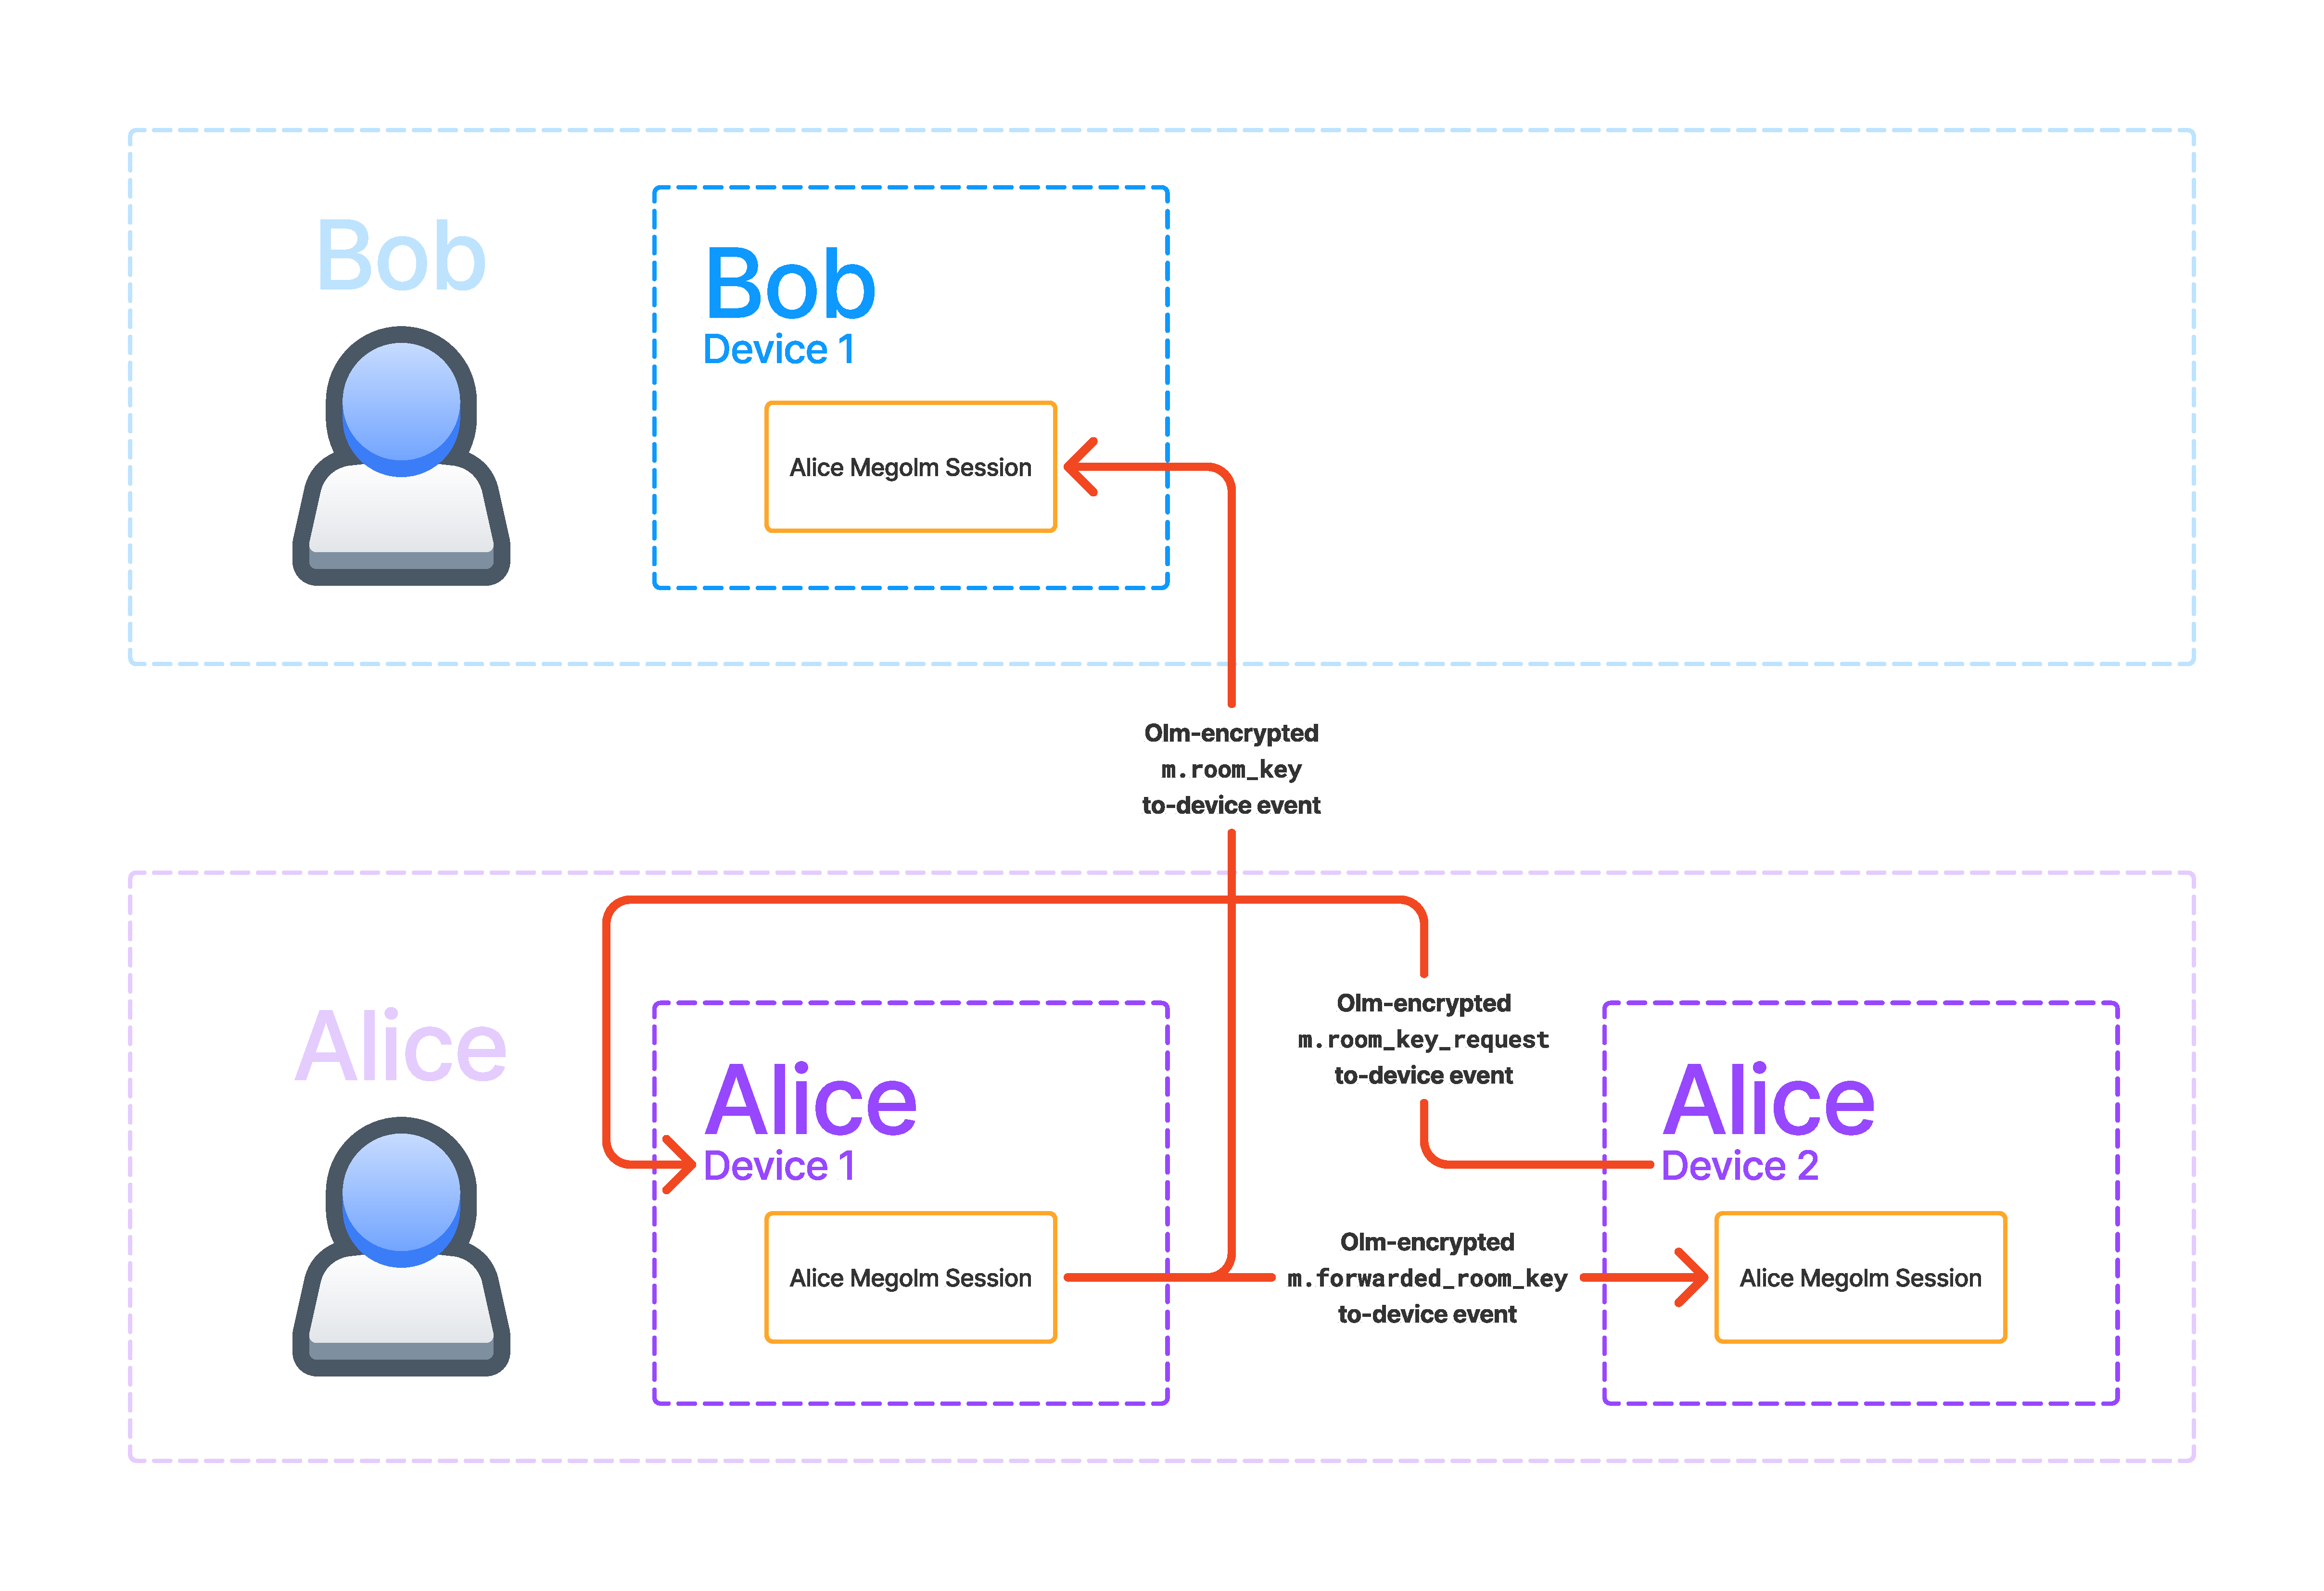
\includegraphics[width=\textwidth]{images/to-device-zoomed}

    \note[item]{
        I'm not going to discuss how Olm encryption works. It's already been
        covered many times since it's basically just the Signal double-ratchet
        algorithm.
    }

    \note[item]{
        For our purposes, it's sufficient to know that we can send keys securely
        to other users' devices and our own devices using via to-device events
        via Olm. We can also request keys from our own \textbf{verified}
        devices. We will talk about how we know a device is verified later.
    }

    \note[item]{
        This seems great, why do we have anything else?
    }

    \note[item]{
        Well, new logins are the issue. Say Alice just logged in on Device 2 and
        finished verification.

        \begin{itemize}
            \item If Device 1 is \textit{online}, she can send key requests, but
                there's likely going to be a ton of requests due to all of the
                keys in all of the rooms to her Device 1. This will make Device
                1 do a lot of work sending back all the keys.
            \item If Device 1 is \textit{\textbf{off}line}, her send key
                requests won't be answered.
        \end{itemize}
    }
\end{frame}

\begin{frame}{Key Backup}
    \includegraphics[width=\textwidth]{images/other-stuff-key-backup}

    \note[item]{
        That's where \textbf{key backup} comes into play. Key backup allows us
        to store keys on the server, and restore them from our other devices
        without the other devices needing to be online.
    }

    \note[item]{
        Let's zoom in and see what's going on.
    }
\end{frame}

\begin{frame}{Key Backup}
    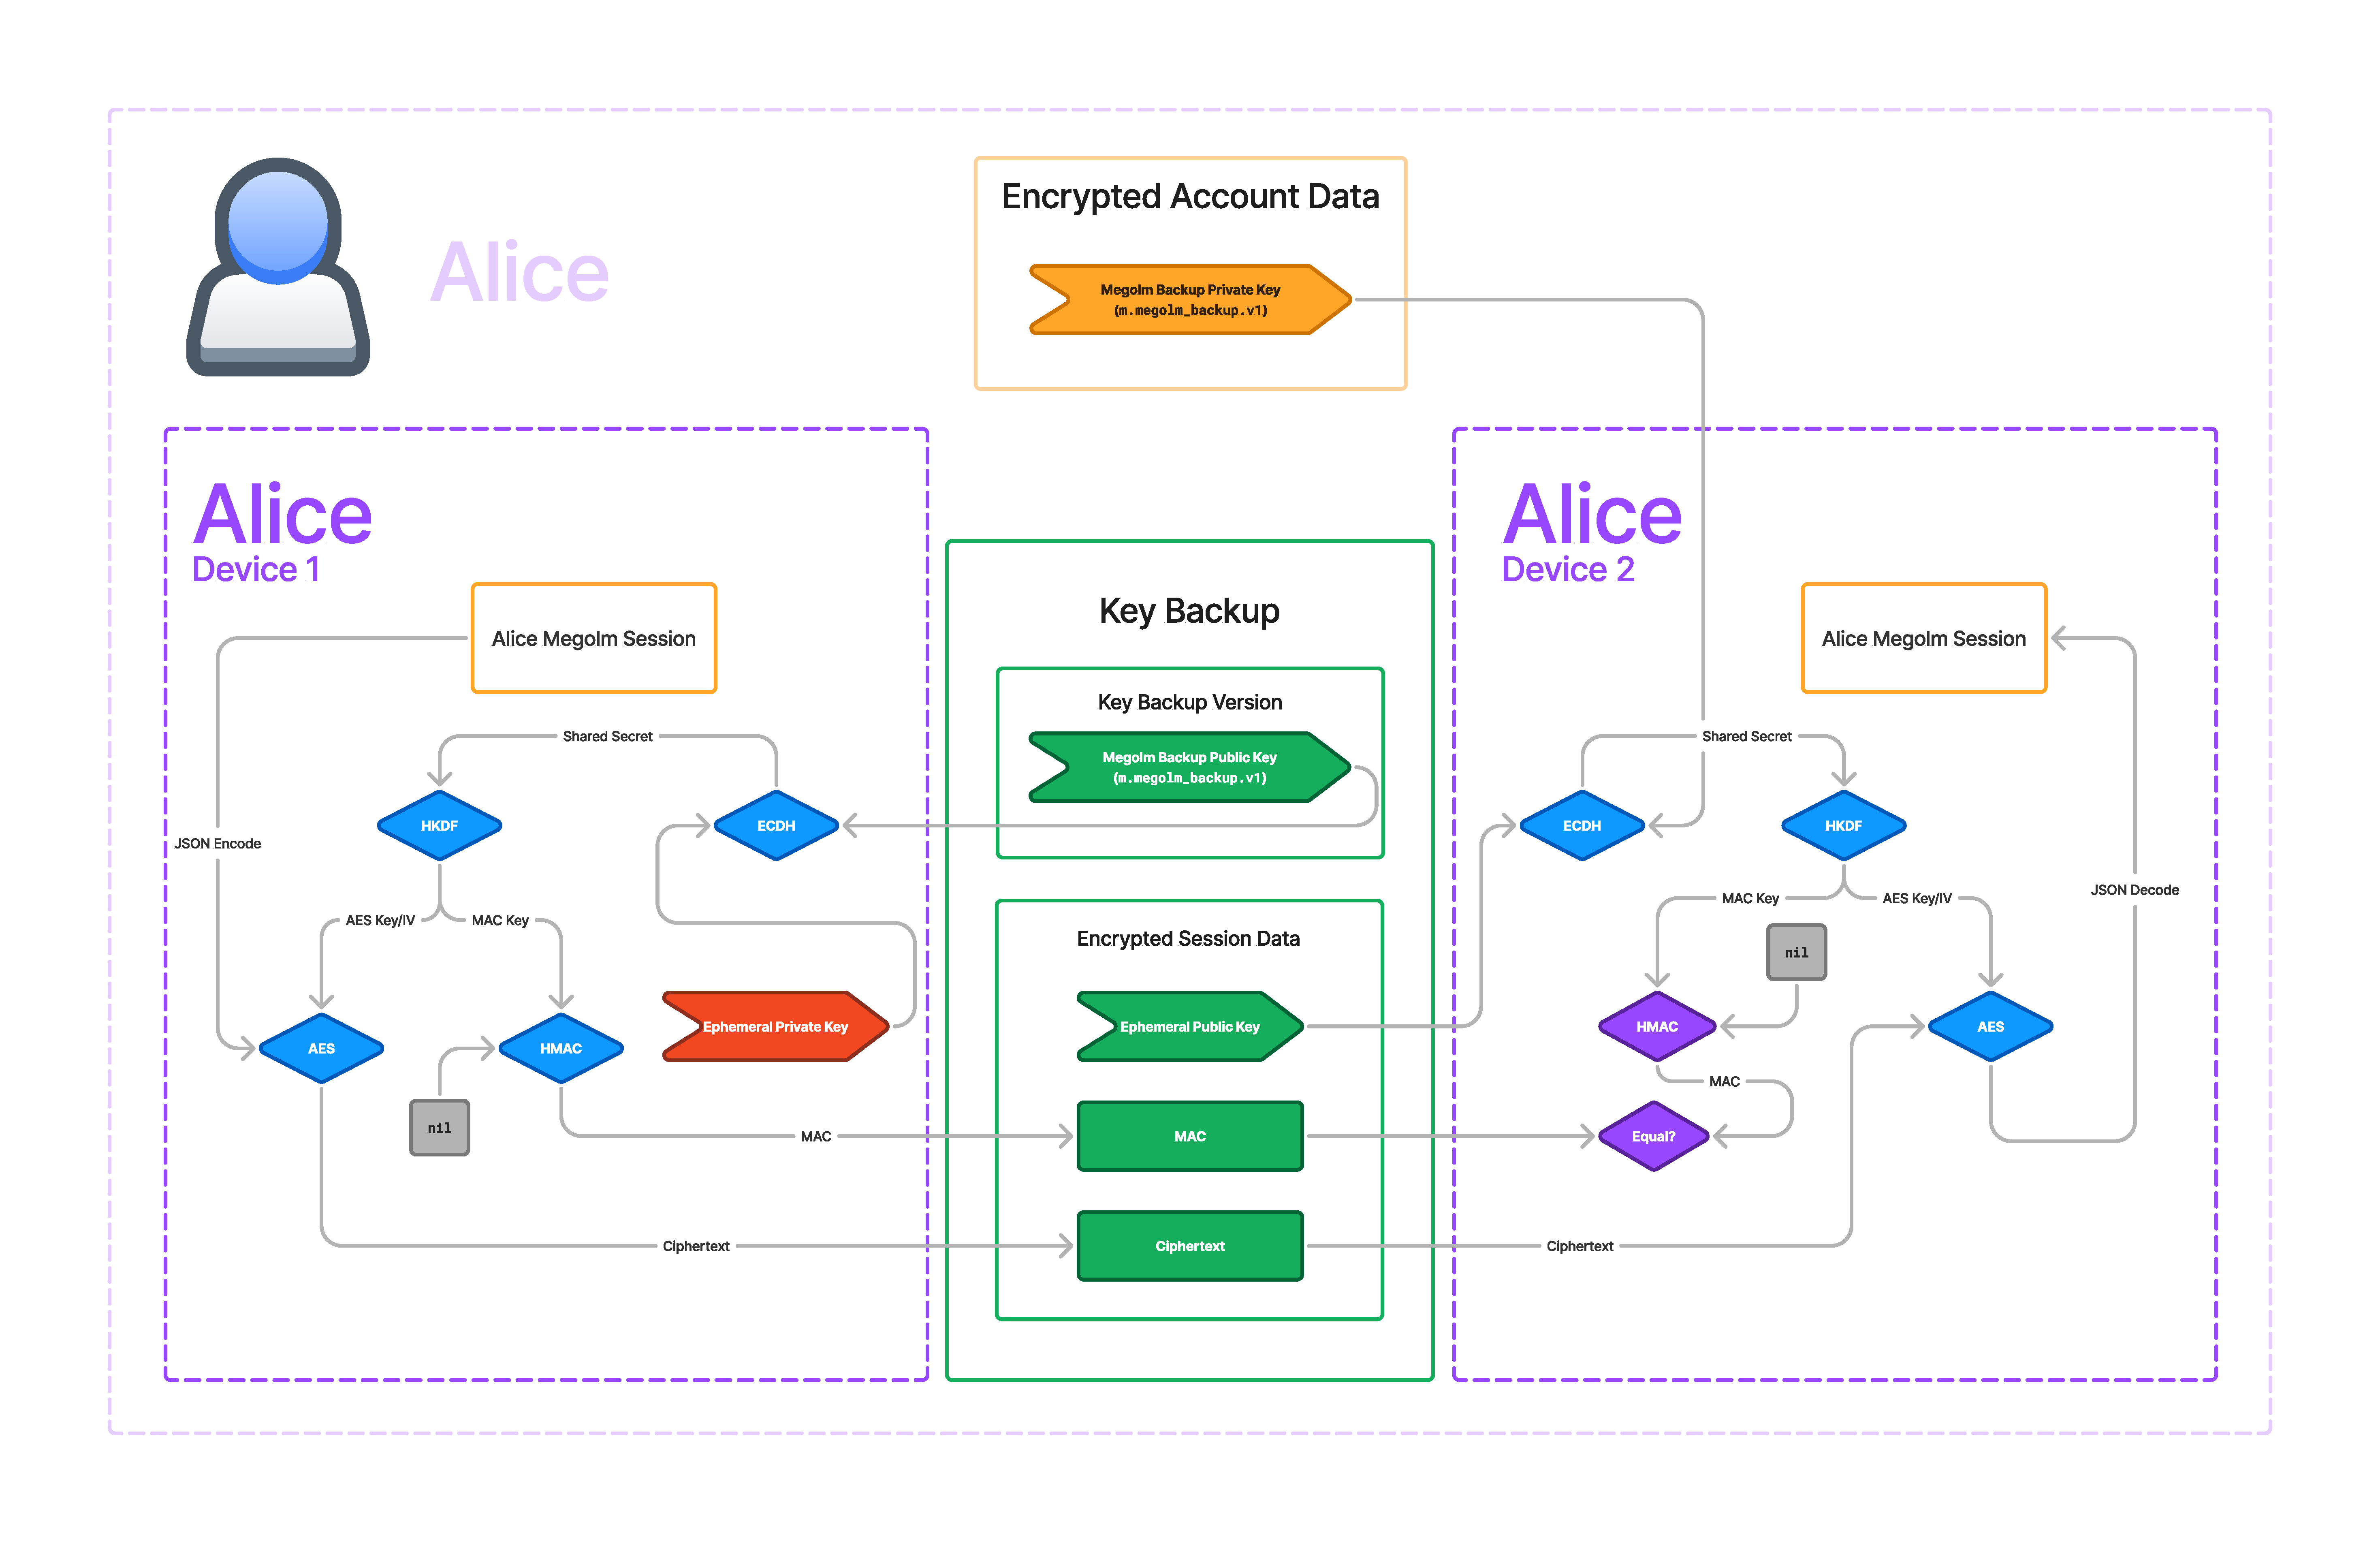
\includegraphics[width=\textwidth]{images/key-backup-zoomed}

    \note[item]{
        In the middle here we have this green ``key backup'' thing which
        is stored on the server. We're trying to get the Megolm key from Alice's
        Device 1 to her Device 2, so left to right.
    }
    \note[item]{
        There are two pieces to key backup:

        \begin{itemize}
            \item the version which includes a public key for the backup.
            \item the encrypted session data (there are many of these in a
                backup (one per megolm session stored)).
        \end{itemize}
    }

    \note[item]{
        The first thing to note is that AES is used on both sides to do the
        encryption and decryption, so only the encrypted version is stored on
        the server. But, where do we get the key and IV from?
    }

    \note[item]{
        Well, we get it from HKDF. So, the next question is where do we get the
        key for HKDF?
    }

    \note[item]{That comes from a call to ECDH.}

    \note[item]{
        Note that all this up to ECDH is \textbf{the same on both the encrypting
        and decrypting sides!}
    }

    \note[item]{
        Recall that ECDH requires a public key and a private key, so where do we
        get those?
    }

    \note[item]{
        This is where the sides diverge.
    }
\end{frame}

\begin{frame}{Key Backup}
    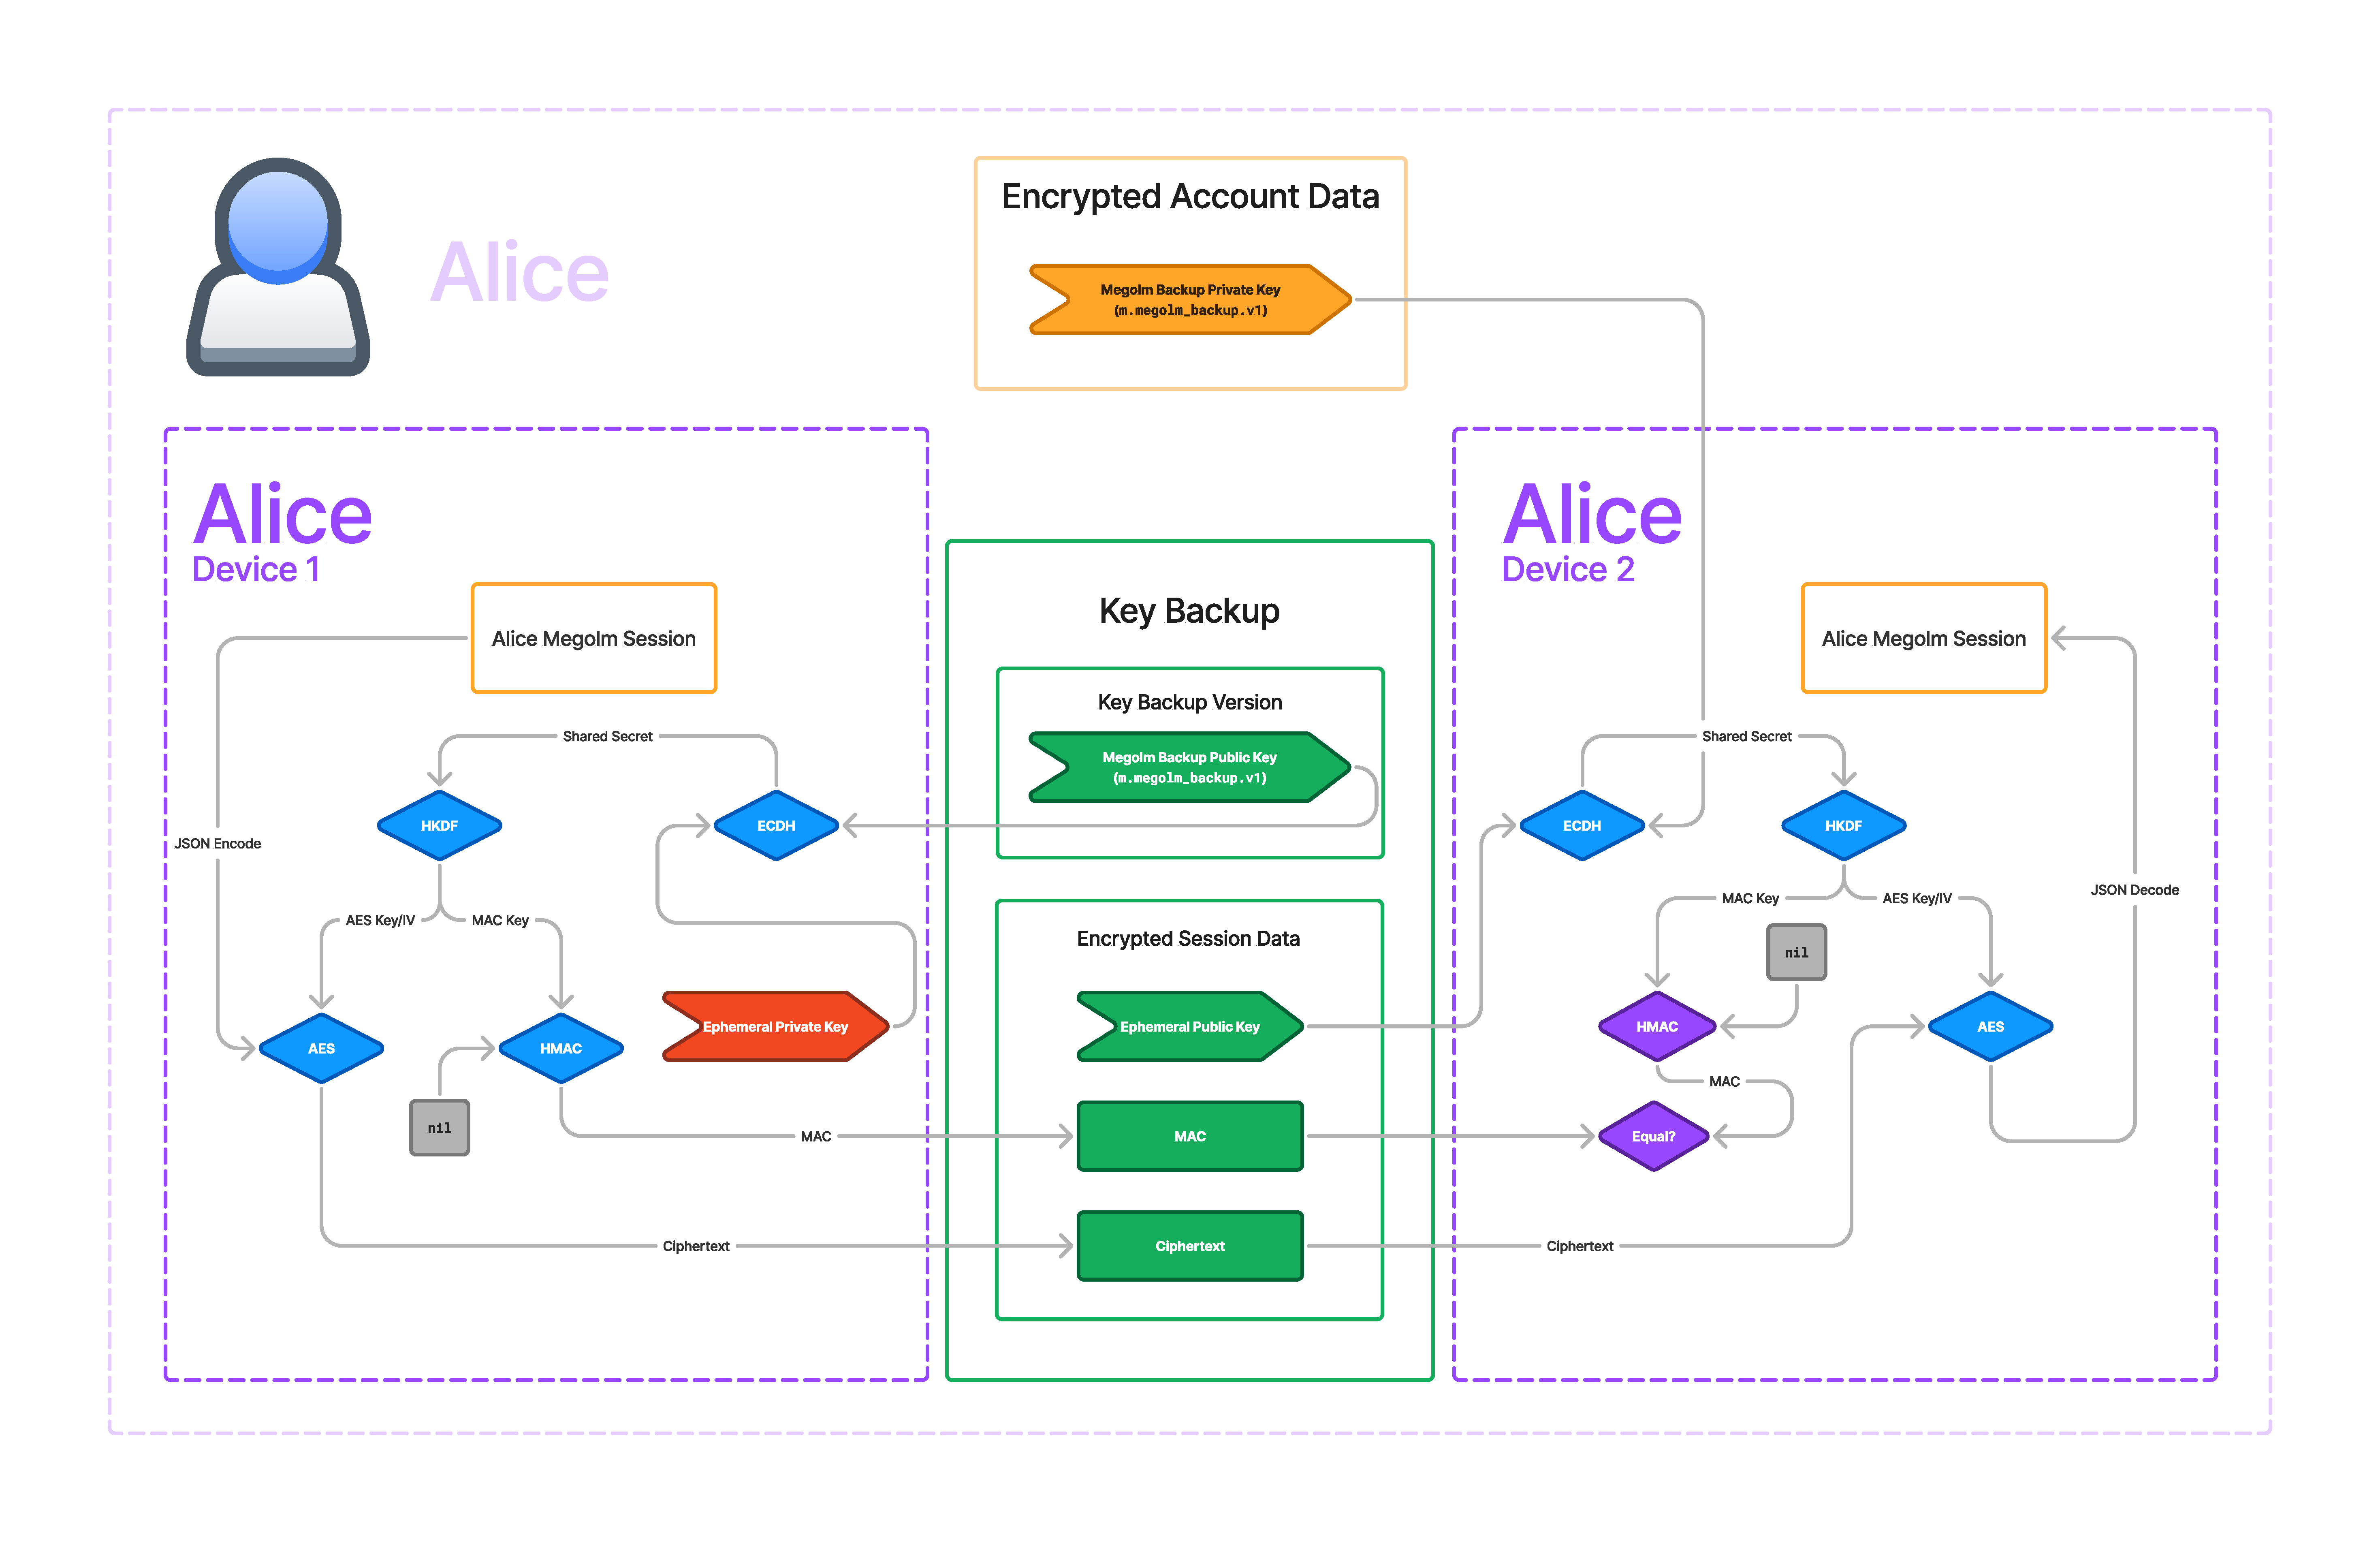
\includegraphics[width=\textwidth]{images/key-backup-zoomed}

    \[
        \textbf{ECDH}(A_{private}, B_{public}) = \textbf{ECDH}(B_{private}, A_{public}) = K_{shared}
    \]

    \note[item]{
        Recall that we need two keypairs for ECDH.
        \begin{itemize}
            \item The first keypair is the Megolm backup keypair.
            \item The second keypair is the Epemeral keypair.
        \end{itemize}
    }

    \note[item]{
        We can use either private key and the other keypair's public key and get
        the same value out of ECDH.

        \begin{itemize}
            \item The encrypting side gets its private key from this
                \textit{ephemeral keypair}. It's ephemeral because the private
                part can be discarded immediately after the encryption is done.

                Thus, it uses the Megolm backup public key as its public key.
            \item The decrypting side gets its private key from the Megolm
                backup private key.

                Thus, it uses the ephemeral public key as its public key.
        \end{itemize}
    }

    \note[item]{
        \textbf{Critically} you must have the Megolm backup private key to
        decrypt the key backup. We will discuss how that is stored later.
    }

    \note[item]{
        For each Megolm session that we back up in key backup, we store the
        ephemeral public key and the ciphertext from AES together in the
        encrypted session data object.
    }

    \note[item]{
        But there's another item that we store in this object: the MAC.
    }

    \note[item]{
        Recall that MACs are meant to ensure that the ciphertext hasn't been
        tampered with by a malicious or incompetent party.
    }

    \note[item]{
        We get the HMAC key from the same HKDF as the AES key and IV.
    }

    \note[item]{
        The other input to HMAC \textit{should} have been the ciphertext.
        However, the original implementation in libolm failed to do this
        correctly and instead just passed an empty buffer, and it has been
        de-facto spec ever since.
    }

    \note[item]{
        So, the MAC is not really useful at all in its current state. I'm hoping
        that a future version of the spec fixes this. Maybe when we get signed
        backups we will get that.
    }
\end{frame}

\section{Device Verification}
\note{
    Now, let's discuss device verification.
}

\begin{frame}{Who Can We Send Keys To?}
    \includegraphics[width=\textwidth]{images/other-stuff-to-device}

    \note[item]{
        Recall how I said that we only want to forward room keys to our
        \textbf{verified} devices?
    }

    \note[item]{
        Now, we are going to discuss how verification status is determined.
    }

    \note[item]{
        The answer is...
    }
\end{frame}

\begin{frame}{Signatures}
    \includegraphics[width=\textwidth]{images/identity-device-verification}

    \note[item]{
        \textbf{Signatures!}
    }

    \note[item]{
        Let's zoom in on this part.
    }

\end{frame}

\begin{frame}{Signatures}
    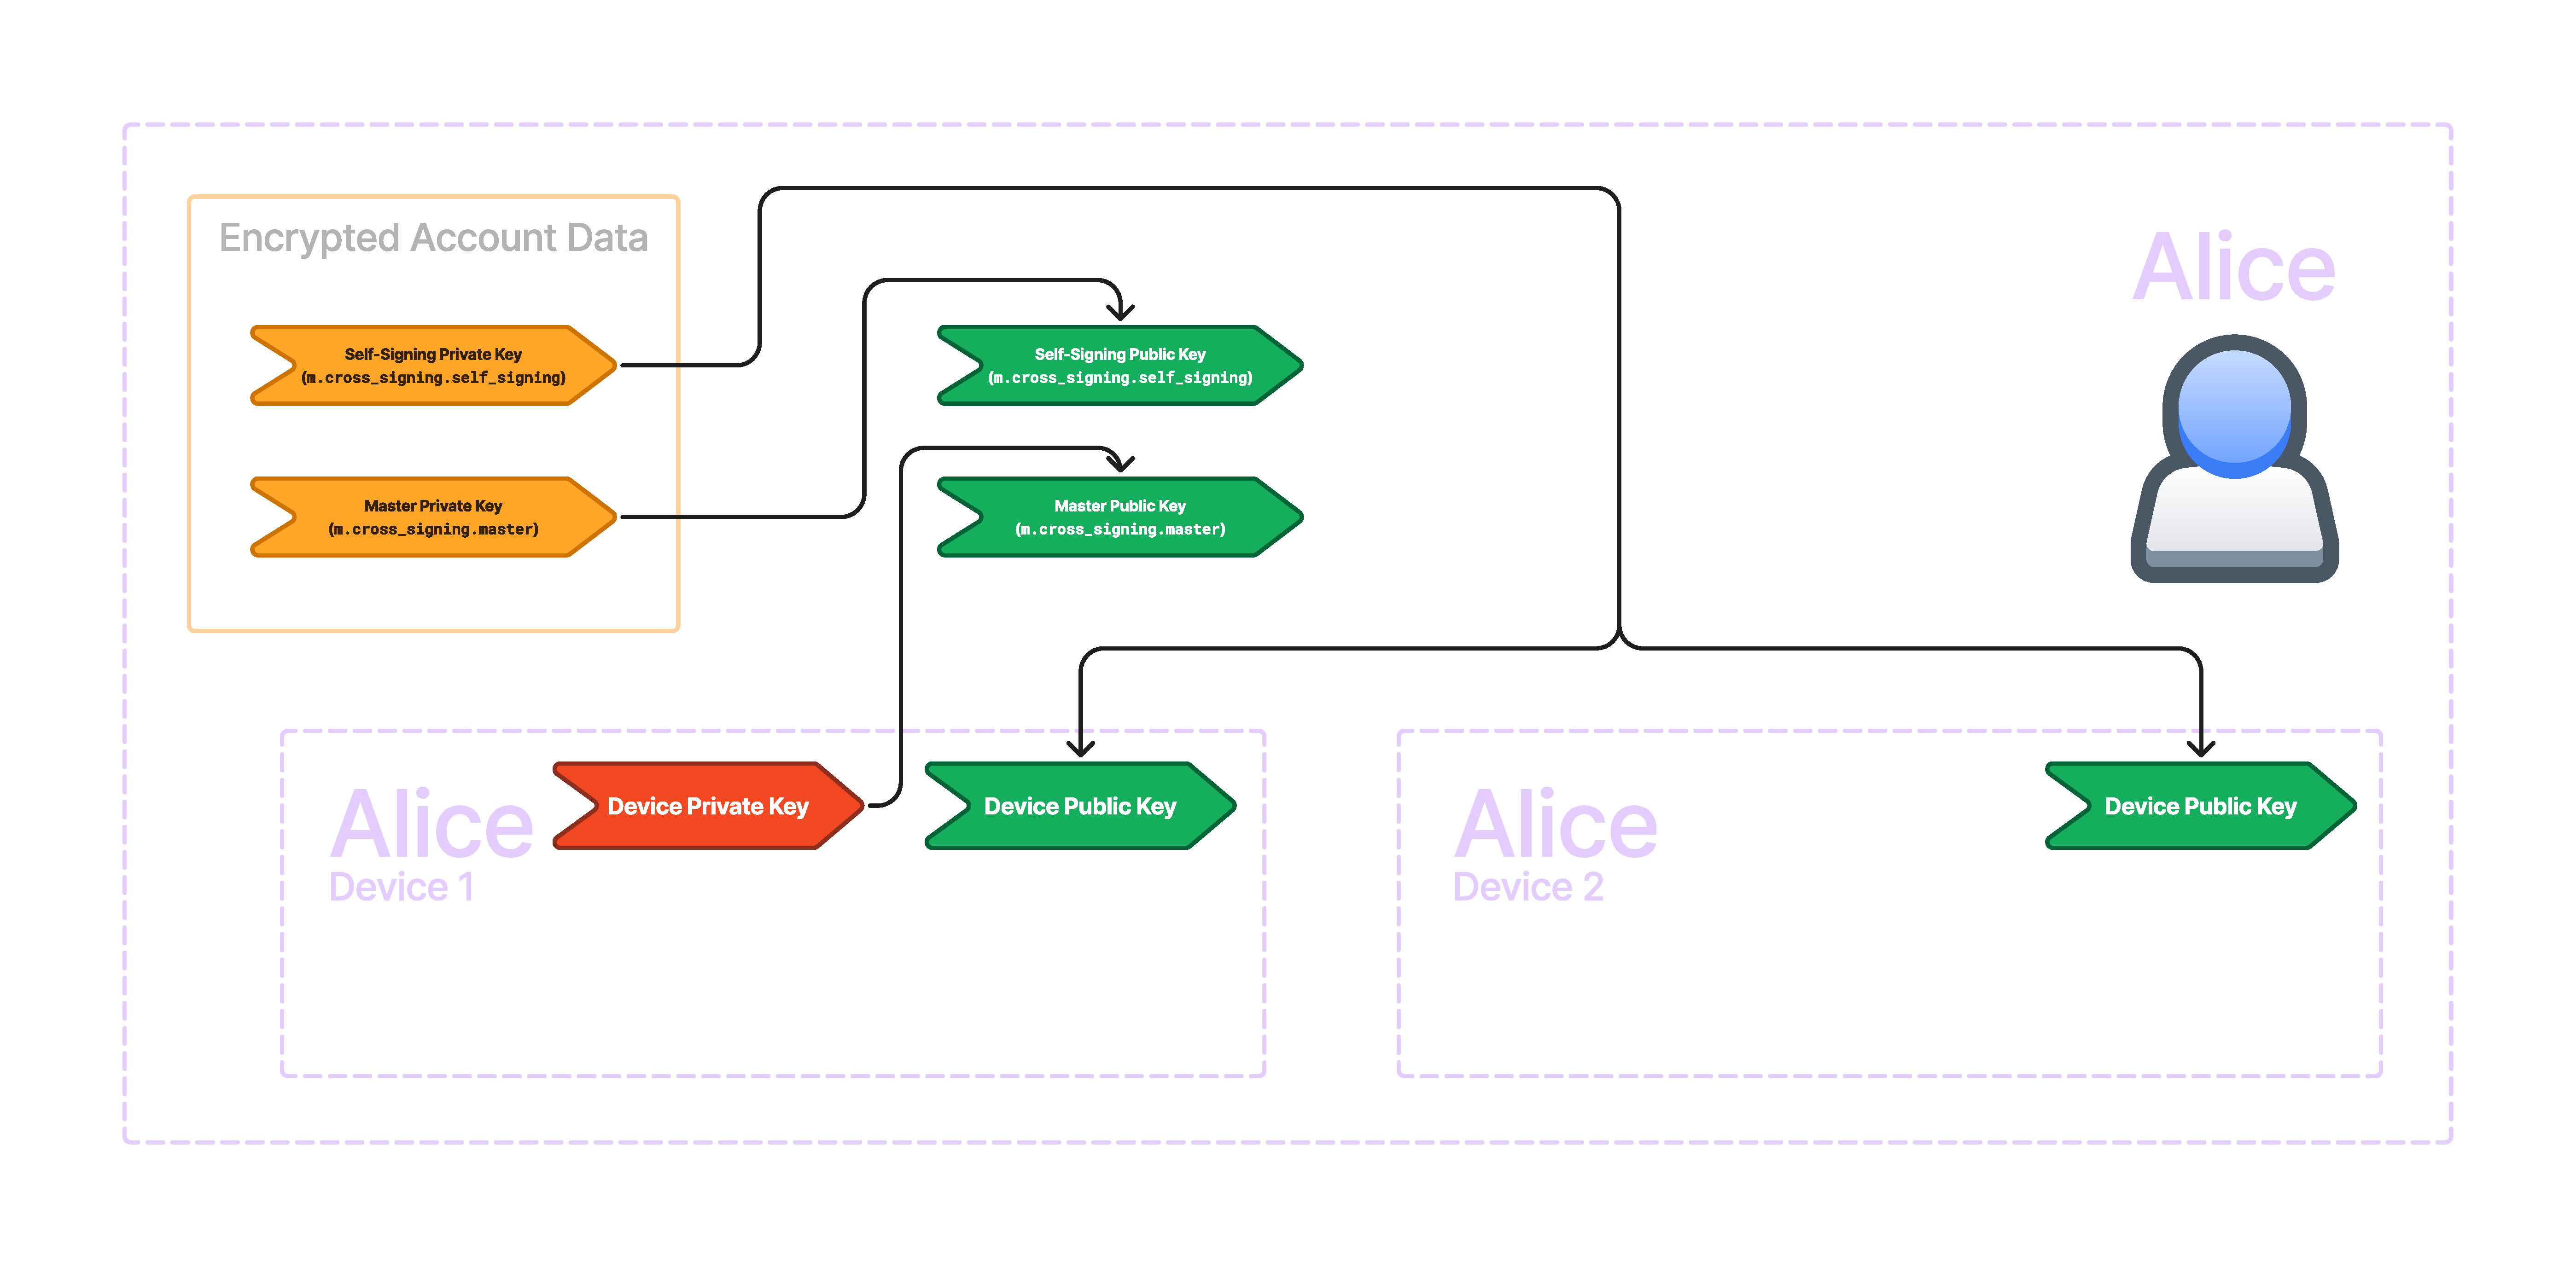
\includegraphics[width=\textwidth]{images/identity-device-verification-zoomed}

    \note[item]{
        Remember, signatures use the \textit{private} key, and anyone who
        possesses the \textit{public} key can verify the signature.
    }

    \note[item]{
        Often, we use ``trust'' terminology. When we ``trust'' a key, we have a
        signature (or chain of signatures) that sign the public key.
    }

    \note[item]{
        Ultimately, the key we want to trust is the other device key.
    }

    \note[item]{
        We can use our device key to directly generate the signature for the
        other device key.

        But that is inconvenient. When we log in a new device, we will have to
        create a signature from all our other devices for that new device. And
        that device will have to create a signature for all of the existing
        devices!
    }

    \note[item]{
        So, we introduce a new user-wide key called the ``self-signing key''
        because it signs our own device keys.
    }

    \note[item]{
        We use the self-signing key to sign the device keys but how do we know
        if we should trust the self-signing key?
    }

    \note[item]{
        That's where the \textbf{master key} comes in. The master key signs the
        self-signing key.
    }

    \note[item]{
        We then trust the master key by signing it with our device private key.
    }

    \note[item]{
        So the \textbf{chain-of-trust} is device private key $\rightarrow$
        master public key which corresponds to its private key $\rightarrow$
        self-signing public key which corresponds to its private key
        $\rightarrow$ device public key.
    }

    \note[item]{
        This allows us to trust a single key (in this case, the master key) and
        then trust all of our own devices.
    }
\end{frame}

\section{User Verification}

\begin{frame}{Additional Identity Verification}
    \includegraphics[width=\textwidth]{images/message-security}

    \note[item]{
        Sometimes, we want to trust a user so that we know that all of the
        devices on their account are under their control. If a new device is
        logged in, we will know if they control the device if it's signed.
    }

    \note[item]{
        They have already signed their devices with their self-signing key,
        which is itself signed by their master key. So, if we are able to trust
        their master key, we will have a chain of trust to all of their devices.
    }

    \note[item]{
        This means that we know that when we send the keys to their devices,
        they are actually under their control.
    }

    \note[item]{
        This is where the ``user-signing key'' comes into play. The user-signing
        key signs other users' master keys and is itself signed by our master
        key.
    }

    \note[item]{
        So the \textbf{chain-of-trust} is device private key $\rightarrow$
        master public key which corresponds to its private key $\rightarrow$
        user-signing public key which corresponds to its private key
        $\rightarrow$ other user's public master key which corresponds to its
        private key $\rightarrow$ other users self-signing key which corresponds
        to its private key $\rightarrow$ other users device public keys.
    }
\end{frame}

\section{Server Side Secret Storage (SSSS)}

\begin{frame}{Don't Forget Your Keys}
    \includegraphics[width=\textwidth]{images/overview.png}

    \note[item]{
        You may have noticed there's a lot of private keys involved in all of
        this.
    }

\end{frame}

\begin{frame}{Don't Forget Your Keys}
    \includegraphics[width=\textwidth]{images/secret-keys-highlighted}

    \note[item]{
        There are private keys for key backup, user signing, and device signing
        and they all need to be stored for all of this to work properly.
    }

    \note[item]{
        The keys are stored each of your devices and can be shared with your
        other verified devices using encrypted to-device events.
    }

    \note[item]{
        But what if you sign out of all of your devices or lose access to them?
    }

\end{frame}

\begin{frame}{Don't Forget Your Keys}
    \includegraphics[width=\textwidth]{images/other-stuff-ssss.png}

    \note[item]{
        That's where server-side secret storage comes in: it allows you to store
        your keys encrypted within account data on the server.
    }

\end{frame}

\begin{frame}{Don't Forget Your Keys}
    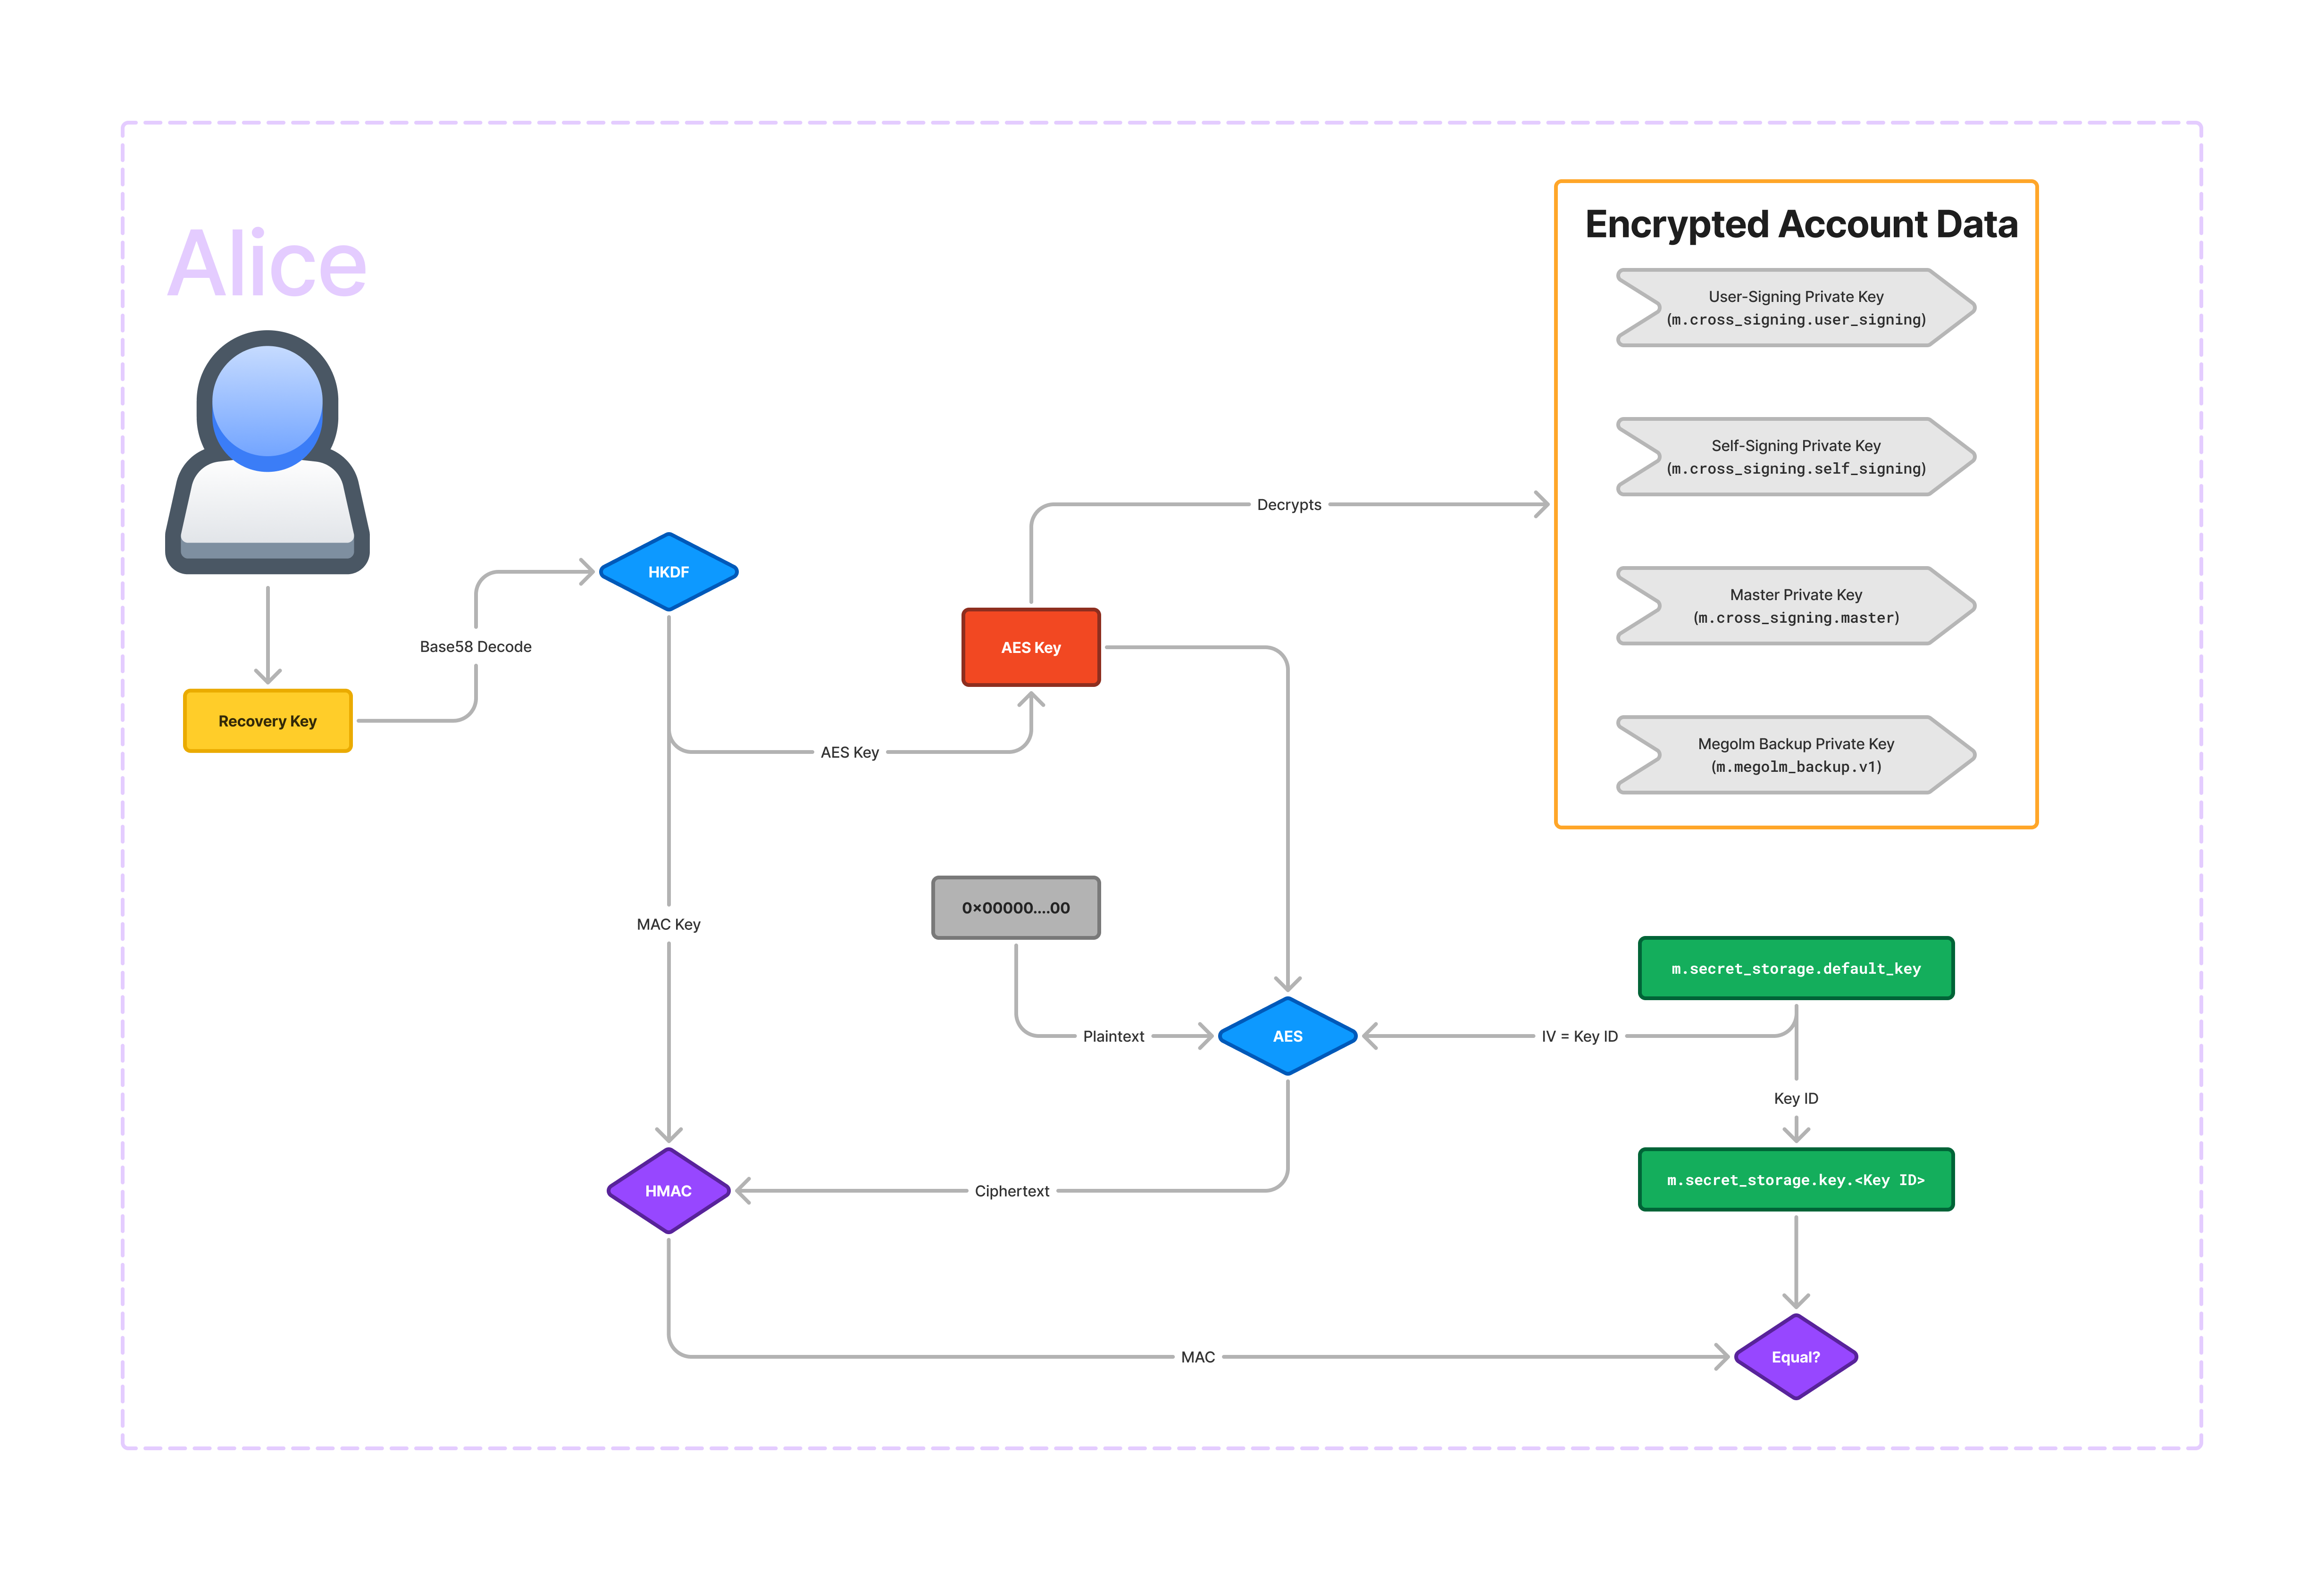
\includegraphics[width=\textwidth]{images/ssss-zoomed.png}

    \note[item]{
        The key that they are encrypted using is basically the recovery key.
        There is an HKDF transformation which gives you the actual key, but it's
        basically just your recovery key that unlocks the encrypted account
        data.
    }

    \note[item]{
        This bottom part isn't actually strictly necessary. It allows you to
        verify that your recovery key is correct. If you want the details here,
        you can read the blog post associated with this talk.
    }

\end{frame}

\begin{frame}{Big Picture}
    \includegraphics[width=\textwidth]{images/overview}

    \note[item]{
        Let's go back to the overview.
    }
    \note[item]{
        We've talked about each piece of this puzzle.
        \begin{itemize}
            \item We talked about to-device events
            \item We talked about key backup
            \item We talked about self-signing of devices
            \item We talked about signing of other users
            \item And then we talked about server-side secret storage
        \end{itemize}
    }
    \note[item]{
        I hope that this presentation has helped you understand how it fits
        together.
    }
    \note[item]{
        My goal is to convince people that Matrix cryptography is not scary.
        It's complex, but not inaccessible.
    }
    \note[item]{
        If you have access to all of the underlying cryptography primitives, all
        of this is something that any security-conscious programmer could
        implement.
    }
    \note[item]{
        You almost certainly should not implement the cryptography primitives
        yourself, but composing them together is not that bad.
    }
    \note[item]{
        And with that, I'll open it up to questions
    }
\end{frame}

\begin{frame}{Thank You for Listening!}
    \center{Questions?}

    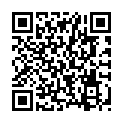
\includegraphics[width=0.5\textwidth]{images/article-qr}
\end{frame}

\end{document}
% Local Variables:
% TeX-command-extra-options: "-shell-escape"
% End:
